
\section{Data products}
\label{sec:products:0}

In the course of this work, we generated several data products, including redshift estimates and a variety of others that can be used to reproduce those estimates and to facilitate thorough evaluation of the algorithm performance.  These products include: configuration files ( Sec.~\ref{sec:products:configuration}), ancillary inputs (Sec.~\ref{sec:products:algo_files}), trained models (Sec.~\ref{sec:products:models}), redshift estimates (Sec.~\ref{sec:products:qp_ensembles}), summary statistics (Sec.~\ref{sec:products:summary_statistics}, and performance monitoring plots (Sec.~\ref{sec:products:peformance_plots}), all of which are essential for understanding the quality of the photometric redshift estimates and for refining the algorithms.   Together, these data products provide a comprehensive framework for conducting, managing, and evaluating photometric redshift estimation workflows in Rubin DP1.  They ensure that the process is not only scientifically rigorous but also organized and reproducible, enabling effective collaboration and ongoing refinement of photometric redshift techniques.


\subsection{Configuration files}
\label{sec:products:configuration}

The configuration files, collected \href{https://github.com/lsstdesc/rail_project_config}{in the GitHub \code{rail\_project\_config}} repository, provide the necessary parameters and settings to control the various stages of the redshift estimation process, are a key element of \code{rail\_projects} workflow.  These files typically include specifications for the photometric bands used (e.g., g, r, i, z), the algorithm choices (e.g., template fitting or machine learning methods), details about data pre-processing, such as feature normalization and handling of missing data.  These configuration files also specify the training and validation dataset splits, hyper-parameters for machine learning models, and paths for input/output data.  These files are essential for ensuring reproducibility and for sharing the exact settings used in different redshift estimation runs, enabling other researchers to replicate or extend the analysis. 


\subsection{Ancillary input files}
\label{sec:products:algo_files}

In addition to the configuration files, we require ancillary inputs such as the galaxy spectral energy distribution (SED) templates and the filter throughputs.  Galaxy SED templates are collections of theoretical or observed spectra for galaxies at different redshifts and with different properties (e.~g.~, galaxy type, age, star formation history).  These templates are used by template-fitting algorithms to model the expected galaxy colors as a function of redshift, allowing for the estimation of photometric redshifts by comparing observed colors to those predicted by the templates.  Two SED sets are employed in this note, they are each described in Section~\ref{sec:method:template}.

The filter throughputs specify the characteristics of the fiducial observational filter transmission curves, and are used in Rubin DP1, including their corresponding central wavelengths.  These filter curves are employed in calculating the synthetic fluxes or magnitudes expected from each of the SED templates used in template-fitting algorithms, and for matching observational data to predicted theoretical values, e.~g.~the predicted colors shown in Figure~\ref{fig:dp_color_v_redshift}.


\subsection{Estimator data models}
\label{sec:products:models}

After training, the trained models for each photometric redshift estimation algorithm are stored as serialized files, either in Pickle (for Python-based models) or YAML (for model configurations) format.  These models encapsulate the learned relationships between photometric features (such as magnitudes and colors) and redshift values, allowing them to be applied to new data for redshift estimation.  These files store the final state of the model, including the weights, biases, and other learned parameters for machine learning models.  In the case of template-fitting methods, the corresponding model files may include the template sets and the fitting parameters.  The Pickle or YAML format ensures that the models can be easily loaded, applied to new datasets, and evaluated in future studies.


\subsection{Redshift estimates stored as QP ensembles}
\label{sec:products:qp_ensembles}

The per-object redshift estimates generated by the photometric redshift algorithms are stored in \code{qp} files.  These files serve as containers for storing the redshift predictions for each object in the dataset before any detailed statistical analysis or final reporting.  In the qp files, each galaxy’s redshift estimate is stored in a format that is compatible with the algorithm providing the estimate.   Specifically, for each object we store distribution $p(z)$, which, depending on the algorithm, maybe represent a posterior probability, a likelihood, a conditional likelihood, or just a hunch as to redshift of the object in question.   These \code{qp} files are designed to be lightweight and easy to query, allowing users to quickly retrieve the redshift estimates for individual objects.  The structure of \code{qp} files is optimized for efficient access and data retrieval, making it easier for users to process and analyze large numbers of photometric redshift estimates across large datasets like Rubin DP1.  Additional information, including usage examples, about \code{qp} and \code{qp} files is available at \href{https://qp.readthedocs.io/en/main/}{https://qp.readthedocs.io/en/main/}.


\subsection{Per-Object Point Estimates}
\label{sec:products:summary_statistics}

In addition to the raw redshift estimates, the \code{qp} files also store per-object point estimates in the form of an ancillary table.  These estimates include crucial information about the quality and reliability of each photometric redshift estimate, such as the uncertainty in the redshift prediction (e.g., the confidence interval or standard deviation or, the likelihood score (in the case of probabilistic models).   This table will eventually includes flags for identifying objects with low-confidence estimates or those that may be outliers.  These summary statistics are important for evaluating the overall performance of the redshift estimation algorithms on an object-by-object basis and are often used to filter out low-quality or problematic redshift estimates before conducting larger statistical analyses.

We also generate meta catalog file that collects the Object ID, magnitude information, and point estimates. The point estimates are named by ``\{algorithm\}\_z\_\{point estimate name\}''.
Here is a list of the point estimates and summary statistics that are stored for each algorithm and the corresponding column names:
\begin{enumerate}
    \item \textbf{mean}: is the per-object expectation of redshift given by the PDF. 
    \item \textbf{median}: is the 50\% percentile of the PDF.
    \item \textbf{mode}: is the redshift that yields maximum PDF evaluated on 301 grid points between $z=0$-$3$. 
    \item \textbf{err68\_lower(upper)}: is the 16th (84th) percentile of the per-galaxy PDF, which correspond to the 1$\sigma$ confidence interval. 
    \item \textbf{err95\_lower(upper)}: is the $2.5$th ($97.5$th) percentile of the per-galaxy PDF, which correspond to the 2$\sigma$ confidence interval. 
\end{enumerate}
Fig.~\ref{fig:pdf} shows an example of the $p(z)$ distribution, point-estimates and summary statistics for a single object.

Yes.\begin{figure*}
    \centering
    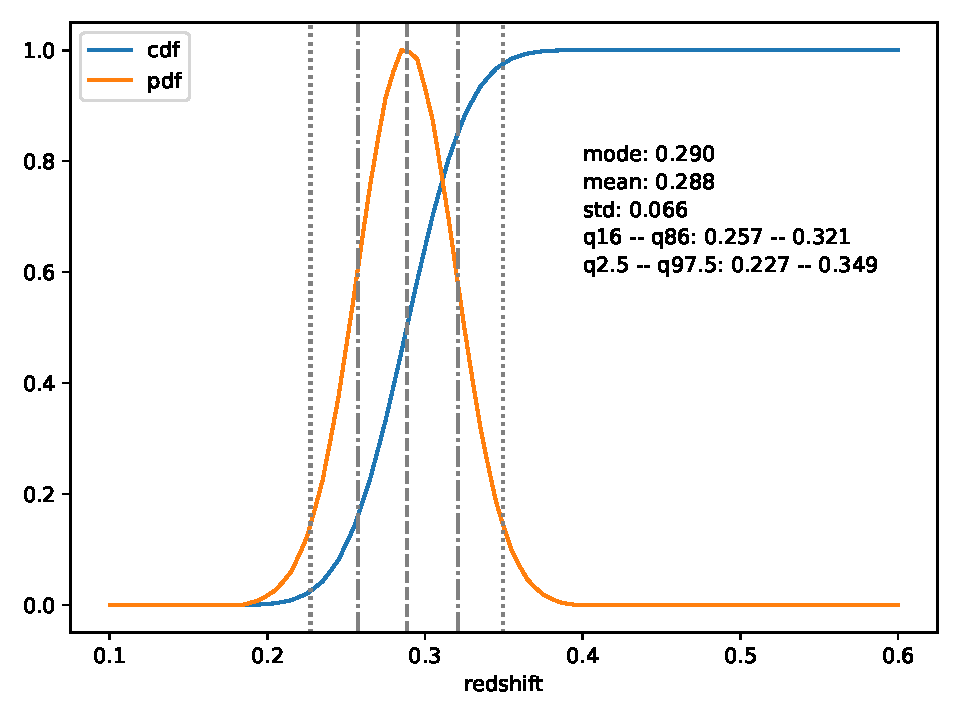
\includegraphics[width=1.0\linewidth]{figures/pdf.pdf}
    \caption{Single object $p(z)$ estimate, showing both the PDF, and the CDF, as well as the summary statistics described in the text.}
    \label{fig:pdf}
\end{figure*}


\subsection{Performance Monitoring Plots}
\label{sec:products:peformance_plots}

Finally, we produced standardized performance monitoring plots as part of the photometric redshift workflow.  These plots provide visual representations of the model's performance, allowing users to assess how well the redshift estimates align with the true redshifts from the spectroscopic training data.  Common plots include:

\begin{itemize}
\item{Input dataset characterization plots, as shown in Sec.~\ref{sec:data:dp1:properties}.}
\item{Scatter plots to visualize the relationship between the predicted and true redshifts, highlighting any systematic biases or non-linearities.}
\item{Redshift comparison plots, e.g., the bias or width of the redshift residuals, $\frac{z_{\rm phot} - z_{\rm spec}}{1 + z_{\rm spec}}$, as a function of redshift or object magnitude.}
\end{itemize}

To robustly summarize the distribution of residuals while minimizing the influence of outliers, we compute biweighted statistics following a two-step procedure. First, we apply an iterative $3\sigma$ clipping to the input array using \texttt{scipy.stats.sigmaclip}, repeating the clipping process \texttt{nclip} times (default is 3). This removes extreme outliers before computing robust estimators. We then calculate the \textit{biweight location} and \textit{biweight scale} of the clipped subset using the \texttt{astropy.stats} functions, which yield robust analogs to the mean and standard deviation, respectively. 

In addition, we compute two outlier rates: the \textit{relative outlier rate}, defined as the fraction of values in the original sample that deviate from zero by more than $3\times$ the biweight scale, and the \textit{absolute outlier rate}, defined as the fraction of values exceeding a fixed threshold set by \texttt{self.config.abs\_out\_thresh}. This framework provides both robust central moments and a diagnostic of extreme deviations in the full sample.

Examples of the two latter types of plots for the \texttt{BPZ} and \texttt{KNN} algorithms are shown in Sec.~\ref{sec:performance:0}


\section{Data Distribution}
\label{sec:distribution:0}

To support both the Rubin community and the DESC, we will distribute these data products in several different ways:
\begin{enumerate}
\item{Via the Rubin Data Butler (see Sec.~\ref{sec:distribution:butler}).}
\item{Via the Photo-z Server (see Sec.~\ref{sec:distribution:linea}).}
\item{Directly as files at the USDF and NERSC (see Sec.~\ref{sec:distribution:files}).}
\item{Via LSDB (see Sec.~\ref{sec:distribution:lsdb})}
\end{enumerate}

In each of these distribution mechanisms there are a number of metadata that are used as fields in defining specific data products.  In particular:

\begin{itemize}
\item{\textbf{algo}: specifies a particular photo-z estimation algorithm (see Tab.~\ref{tab:alg}),}
\item{\textbf{selection}: specifies a particular data selection (see Sec.~\ref{sec:data:dp1:preparation}),}
\item{\textbf{flavor}: specifies a particular set of configuration parameters,}
\item{\textbf{dataset}: specifies a particular dataset (see Sec.~\ref{tab:dataset}).}
\item{\textbf{version}: specifies a processing version (e.g., v1, v2).}
\end{itemize}


\subsection{Distribution via the Rubin Data Butler}
\label{sec:distribution:butler}

Creation of photometric redshift estimates using RAIL in the Rubin DM framework and distribution via the Rubin Data Butler is supported the \href{https://github.com/lsst-dm/meas_pz}{\code{meas\_pz}} software package for DM supported algorithms and by the \href{https://github.com/lsst-dm/meas_pz}{\code{meas\_pz\_extensions}} software package for the community-supported algorithms described in this note.

For DP1, the following objects stored in the data butler at USDF and NERSC are listed in Tab.~\ref{tab:butler}.

\begin{table*}
\centering
\begin{tabular}{ll}
 \hline
Dataset type & Description \\
 \hline
 \hline
\multicolumn{2}{l}{Collection: \code{pretrained\_models/pz/DP1/\{selection\}/\{flavor\}}} \\ \hline
\code{pzModel\_\{algo\}} & Estimator models (see ~\ref{sec:products:models}) \\ \hline
\multicolumn{2}{l}{Collection: \code{LSSTComCam/runs/DRP/DP1/pz/DM-51523/\{selection\}/\{flavor\}/\{version\}}} \\  \hline
\code{pz\_estimate\_\{algo\}} & QP ensembles (see ~\ref{sec:products:qp_ensembles}) \\
\code{pz\_\{algo\}\_config} & Configuration parameters (see ~\ref{sec:products:configuration}) \\
\code{pz\_\{algo\}\_log} & Log files \\
\code{pz\_\{algo\}\_metadata} & Processing metadata \\
 \hline
\end{tabular}
\caption{Photo-z related objects stored in the Rubin Data Butler.  Note that \code{\{selection\}} describes the selection applied to the trained data set.}
\label{tab:butler}
\end{table*}


\subsection{Distribution via the Photo-z Server}
\label{sec:distribution:linea}
% Julia

The \href{https://pzserver.linea.org.br/}{Photo-z Server (or PZ Server)} is a web-based service available for the LSST community to create and host PZ-related lightweight data products. It relies on the infrastructure of the Brazilian Independent Data Access Center and is developed and maintained by LIneA as part of the Brazilian in-kind contribution program.  

The PZ server is open to any LSST member with a valid RSP account without the need for an extra local registry. Users can log into the system simply using the RSP credentials. 

All data products described in this document 
will be % are also 
hosted on the PZ Server, along with their respective metadata and documentation. There are two ways to access these data products: 

\subsubsection{From the PZ Server website} 

Data products are listed both on the 'Rubin PZ Data Products' page (for official data products released or recommended by LSST DM) and 'User-generated data products' for data products produced or uploaded by the LSST community members. The DP1 PZ data products described in this document
will be 
%are 
available in the first one. %, and their links to individual data product details pages are listed below: 

% \begin{itemize}
%     \item Spec-z Catalog \href{https://pzserver-dev.linea.org.br/}{<product name placeholder>}
%     \item Training and Test Sets \href{https://pzserver-dev.linea.org.br/}{<product name placeholder>}
%     \item Estimator Data Models \href{https://pzserver-dev.linea.org.br/}{<product name placeholder>}
%     \item Redshift estimates \href{https://pzserver-dev.linea.org.br/}{<product name placeholder>}
% \end{itemize} 

\subsubsection{Via the \code{pzserver} Python library}

Similar to the RSP, the PZ Server provides an API interface that enables users to access data through Python scripts from any location, provided they know the product name as registered on the server. 
 
If it is the first time using the library, it must be installed via \code{pip} in the terminal or in a notebook cell: \code{pip install pzserver}

Then, the \code{PzServer} class opens the remote connection to the PZ Server database. An access token is required for authentication. The token can be generated by users on the PZ Server website (top right corner menu on the home page).    

\begin{verbatim}
from pzserver import PzServer
pz_server = PzServer(token="<paste your access token here>")  
\end{verbatim}

To display the product metadata and download it to the local working directory (if not in a Jupyter notebook, replace \code{display} for \code{get}):   
\begin{verbatim}
pz_server.display_product_metadata(<product_id>)
pz_server.download_product(product_id, save_in=".")
\end{verbatim}

Alternatively, it is possible to load a table directly into memory as a Pandas DataFrame or Astropy Table. For instance, to load a training set:  

\begin{verbatim}
training_set = pz_server.get_product(<training_set_id>)
training_set.display_metadata()
\end{verbatim}

%%%%%%%%%%%%%%%%%%%%%%%%%%%%%%%%%%%%%%%%%%
% TO DO: 
% Add examples with the correct product_id 
% of datasets mentioned in this document
%%%%%%%%%%%%%%%%%%%%%%%%%%%%%%%%%%%%%%%%%%

A tutorial notebook with examples for all \code{pzserver} methods is available on the \href{https://github.com/linea-it/pzserver/blob/main/docs/notebooks/pzserver_tutorial.ipynb}{\code{pzserver} library's repository on GitHub}.


\subsection{Distribution as files at USDF and NERSC}
\label{sec:distribution:files}

All of the test and training files, the outputs from runs used to optimize the model hyperparamters, as well as from the optimized models, the photo-z estimates for the entire DP1 dataset, are all available in \code{rail\_projects}-managed shared project area at both NERSC and USDF.  These data products are listed in Tab.~\ref{tab:project_area}.

\begin{table*}
\centering
\begin{tabular}{ll}
 \hline
Object type  & Relative Path \\
 \hline
 \hline
Training data sets  & \code{data/train/*.hdf5} \\ 
Test data sets  & \code{data/test/*.hdf5} \\ \hline
\multicolumn{2}{l}{In : \code{pz/projects/dp1/pipelines}} \\ \hline
Pipeline configurations & \code{\{pipeline\}\_\{flavor\}.yaml} \\ \hline
\multicolumn{2}{l}{In : \code{pz/projects/dp1/data}} \\ \hline
Estimator models & \code{\{selection\}\_\{flavor\}/model\_inform\_\{algo\}.pkl} \\
QP ensembles (for test data) & \code{\{selection\}\_\{flavor\}/output\_estimate\_\{algo\}.hdf5} \\
QP ensembles (for other data) & \code{\{selection\}\_\{flavor\}/\{dataset\}/output\_estimate\_\{algo\}.hdf5} \\
 \hline
\end{tabular}
\caption{Photo-z related files in the \code{rail\_projects}-managed shared project areas.}
\label{tab:project_area}
\end{table*}


\subsection{Distribution via LSDB}
\label{sec:distribution:lsdb}

The Large Survey DataBase (LSDB) will host the DP1 data on the USDF and the Canadian IDAC RSP. The DP1 data will be turned into Hierarchical Adaptive Tiling Scheme (HATS) format. LSDB enables researchers to load large datasets with limited memory, and fast cross match to other surveys like DESI DR1 and GAIA DR3. 

The photo-z point estimates for DP1 in the \field{ECDFS},\field{EDFS}, \field{Rubin\_SV\_95\_-25}, and \field{Rubin\_SV\_38\_7}  will be served as a single tabular catalog in the LSDB. The location on the USDF for this catalog is \texttt{/sdf/data/rubin/shared/lsdb\_commissioning/dp1\_pz\_hats}. 


\pagebreak

%  LocalWords:  fig:dp_color_v_redshift qp qp qp qp qp qp textbf th
%  LocalWords:  th includegraphics linewidth biweighted texttt nclip
%  LocalWords:  textit biweight textit biweight _pz hline pretrained
%  LocalWords:  pzModel pz subsubsection pzserver Astropy hdf5 pkl
%  LocalWords:  hyperparamters
